% Options for packages loaded elsewhere
\PassOptionsToPackage{unicode}{hyperref}
\PassOptionsToPackage{hyphens}{url}
\PassOptionsToPackage{dvipsnames,svgnames,x11names}{xcolor}
%
\documentclass[
  nobib]{ccr}

% [WvA] change from original template.tex - amssymb is replaced by / clashes with newtxmath]
% \usepackage{amsmath,amssymb}
\usepackage{amsmath}

\usepackage{iftex}
\ifPDFTeX
  \usepackage[T1]{fontenc}
  \usepackage[utf8]{inputenc}
  \usepackage{textcomp} % provide euro and other symbols
\else % if luatex or xetex
  % [WvA] change from original template.tex - unicode-math is replaced by / clashes with newtxmath]
  %% \usepackage{unicode-math}
  \defaultfontfeatures{Scale=MatchLowercase}
  \defaultfontfeatures[\rmfamily]{Ligatures=TeX,Scale=1}
\fi
% Use upquote if available, for straight quotes in verbatim environments
\IfFileExists{upquote.sty}{\usepackage{upquote}}{}
\IfFileExists{microtype.sty}{% use microtype if available
  \usepackage[]{microtype}
  \UseMicrotypeSet[protrusion]{basicmath} % disable protrusion for tt fonts
}{}
\makeatletter
\@ifundefined{KOMAClassName}{% if non-KOMA class
  \IfFileExists{parskip.sty}{%
    \usepackage{parskip}
  }{% else
    \setlength{\parindent}{0pt}
    \setlength{\parskip}{6pt plus 2pt minus 1pt}}
}{% if KOMA class
  \KOMAoptions{parskip=half}}
\makeatother
\usepackage{xcolor}
\setlength{\emergencystretch}{3em} % prevent overfull lines
\setcounter{secnumdepth}{-\maxdimen} % remove section numbering
% Make \paragraph and \subparagraph free-standing
\ifx\paragraph\undefined\else
  \let\oldparagraph\paragraph
  \renewcommand{\paragraph}[1]{\oldparagraph{#1}\mbox{}}
\fi
\ifx\subparagraph\undefined\else
  \let\oldsubparagraph\subparagraph
  \renewcommand{\subparagraph}[1]{\oldsubparagraph{#1}\mbox{}}
\fi
\usepackage{color}
\usepackage{fancyvrb}
\newcommand{\VerbBar}{|}
\newcommand{\VERB}{\Verb[commandchars=\\\{\}]}
\DefineVerbatimEnvironment{Highlighting}{Verbatim}{commandchars=\\\{\}}
% Add ',fontsize=\small' for more characters per line
\usepackage{framed}
\definecolor{shadecolor}{RGB}{241,243,245}
\newenvironment{Shaded}{\begin{snugshade}}{\end{snugshade}}
\newcommand{\AlertTok}[1]{\textcolor[rgb]{0.68,0.00,0.00}{#1}}
\newcommand{\AnnotationTok}[1]{\textcolor[rgb]{0.37,0.37,0.37}{#1}}
\newcommand{\AttributeTok}[1]{\textcolor[rgb]{0.40,0.45,0.13}{#1}}
\newcommand{\BaseNTok}[1]{\textcolor[rgb]{0.68,0.00,0.00}{#1}}
\newcommand{\BuiltInTok}[1]{\textcolor[rgb]{0.00,0.23,0.31}{#1}}
\newcommand{\CharTok}[1]{\textcolor[rgb]{0.13,0.47,0.30}{#1}}
\newcommand{\CommentTok}[1]{\textcolor[rgb]{0.37,0.37,0.37}{#1}}
\newcommand{\CommentVarTok}[1]{\textcolor[rgb]{0.37,0.37,0.37}{\textit{#1}}}
\newcommand{\ConstantTok}[1]{\textcolor[rgb]{0.56,0.35,0.01}{#1}}
\newcommand{\ControlFlowTok}[1]{\textcolor[rgb]{0.00,0.23,0.31}{\textbf{#1}}}
\newcommand{\DataTypeTok}[1]{\textcolor[rgb]{0.68,0.00,0.00}{#1}}
\newcommand{\DecValTok}[1]{\textcolor[rgb]{0.68,0.00,0.00}{#1}}
\newcommand{\DocumentationTok}[1]{\textcolor[rgb]{0.37,0.37,0.37}{\textit{#1}}}
\newcommand{\ErrorTok}[1]{\textcolor[rgb]{0.68,0.00,0.00}{#1}}
\newcommand{\ExtensionTok}[1]{\textcolor[rgb]{0.00,0.23,0.31}{#1}}
\newcommand{\FloatTok}[1]{\textcolor[rgb]{0.68,0.00,0.00}{#1}}
\newcommand{\FunctionTok}[1]{\textcolor[rgb]{0.28,0.35,0.67}{#1}}
\newcommand{\ImportTok}[1]{\textcolor[rgb]{0.00,0.46,0.62}{#1}}
\newcommand{\InformationTok}[1]{\textcolor[rgb]{0.37,0.37,0.37}{#1}}
\newcommand{\KeywordTok}[1]{\textcolor[rgb]{0.00,0.23,0.31}{\textbf{#1}}}
\newcommand{\NormalTok}[1]{\textcolor[rgb]{0.00,0.23,0.31}{#1}}
\newcommand{\OperatorTok}[1]{\textcolor[rgb]{0.37,0.37,0.37}{#1}}
\newcommand{\OtherTok}[1]{\textcolor[rgb]{0.00,0.23,0.31}{#1}}
\newcommand{\PreprocessorTok}[1]{\textcolor[rgb]{0.68,0.00,0.00}{#1}}
\newcommand{\RegionMarkerTok}[1]{\textcolor[rgb]{0.00,0.23,0.31}{#1}}
\newcommand{\SpecialCharTok}[1]{\textcolor[rgb]{0.37,0.37,0.37}{#1}}
\newcommand{\SpecialStringTok}[1]{\textcolor[rgb]{0.13,0.47,0.30}{#1}}
\newcommand{\StringTok}[1]{\textcolor[rgb]{0.13,0.47,0.30}{#1}}
\newcommand{\VariableTok}[1]{\textcolor[rgb]{0.07,0.07,0.07}{#1}}
\newcommand{\VerbatimStringTok}[1]{\textcolor[rgb]{0.13,0.47,0.30}{#1}}
\newcommand{\WarningTok}[1]{\textcolor[rgb]{0.37,0.37,0.37}{\textit{#1}}}

\usepackage{longtable,booktabs,array}
\newcounter{none} % for unnumbered tables
\usepackage{calc} % for calculating minipage widths
% Correct order of tables after \paragraph or \subparagraph
\usepackage{etoolbox}
\makeatletter
\patchcmd\longtable{\par}{\if@noskipsec\mbox{}\fi\par}{}{}
\makeatother
% Allow footnotes in longtable head/foot
\IfFileExists{footnotehyper.sty}{\usepackage{footnotehyper}}{\usepackage{footnote}}
\makesavenoteenv{longtable}
\usepackage{graphicx}
\makeatletter
\newsavebox\pandoc@box
\newcommand*\pandocbounded[1]{% scales image to fit in text height/width
  \sbox\pandoc@box{#1}%
  \Gscale@div\@tempa{\textheight}{\dimexpr\ht\pandoc@box+\dp\pandoc@box\relax}%
  \Gscale@div\@tempb{\linewidth}{\wd\pandoc@box}%
  \ifdim\@tempb\p@<\@tempa\p@\let\@tempa\@tempb\fi% select the smaller of both
  \ifdim\@tempa\p@<\p@\scalebox{\@tempa}{\usebox\pandoc@box}%
  \else\usebox{\pandoc@box}%
  \fi%
}
% Set default figure placement to htbp
\def\fps@figure{htbp}
\makeatother


% definitions for citeproc citations
\NewDocumentCommand\citeproctext{}{}
\NewDocumentCommand\citeproc{mm}{%
  \begingroup\def\citeproctext{#2}\cite{#1}\endgroup}
\makeatletter
 % allow citations to break across lines
 \let\@cite@ofmt\@firstofone
 % avoid brackets around text for \cite:
 \def\@biblabel#1{}
 \def\@cite#1#2{{#1\if@tempswa , #2\fi}}
\makeatother
\newlength{\cslhangindent}
\setlength{\cslhangindent}{1.5em}
\newlength{\csllabelwidth}
\setlength{\csllabelwidth}{3em}
\newenvironment{CSLReferences}[2] % #1 hanging-indent, #2 entry-spacing
 {\begin{list}{}{%
  \setlength{\itemindent}{0pt}
  \setlength{\leftmargin}{0pt}
  \setlength{\parsep}{0pt}
  % turn on hanging indent if param 1 is 1
  \ifodd #1
   \setlength{\leftmargin}{\cslhangindent}
   \setlength{\itemindent}{-1\cslhangindent}
  \fi
  % set entry spacing
  \setlength{\itemsep}{#2\baselineskip}}}
 {\end{list}}
\usepackage{calc}
\newcommand{\CSLBlock}[1]{\hfill\break\parbox[t]{\linewidth}{\strut\ignorespaces#1\strut}}
\newcommand{\CSLLeftMargin}[1]{\parbox[t]{\csllabelwidth}{\strut#1\strut}}
\newcommand{\CSLRightInline}[1]{\parbox[t]{\linewidth - \csllabelwidth}{\strut#1\strut}}
\newcommand{\CSLIndent}[1]{\hspace{\cslhangindent}#1}



\setlength{\emergencystretch}{3em} % prevent overfull lines

\providecommand{\tightlist}{%
  \setlength{\itemsep}{0pt}\setlength{\parskip}{0pt}}



 


\AddToHook{env/Highlighting/begin}{\scriptsize \linespread{1}}
\makeatletter
\@ifpackageloaded{caption}{}{\usepackage{caption}}
\AtBeginDocument{%
\ifdefined\contentsname
  \renewcommand*\contentsname{Table of contents}
\else
  \newcommand\contentsname{Table of contents}
\fi
\ifdefined\listfigurename
  \renewcommand*\listfigurename{List of Figures}
\else
  \newcommand\listfigurename{List of Figures}
\fi
\ifdefined\listtablename
  \renewcommand*\listtablename{List of Tables}
\else
  \newcommand\listtablename{List of Tables}
\fi
\ifdefined\figurename
  \renewcommand*\figurename{Figure}
\else
  \newcommand\figurename{Figure}
\fi
\ifdefined\tablename
  \renewcommand*\tablename{Table}
\else
  \newcommand\tablename{Table}
\fi
}
\@ifpackageloaded{float}{}{\usepackage{float}}
\floatstyle{ruled}
\@ifundefined{c@chapter}{\newfloat{codelisting}{h}{lop}}{\newfloat{codelisting}{h}{lop}[chapter]}
\floatname{codelisting}{Listing}
\newcommand*\listoflistings{\listof{codelisting}{List of Listings}}
\makeatother
\makeatletter
\makeatother
\makeatletter
\@ifpackageloaded{caption}{}{\usepackage{caption}}
\@ifpackageloaded{subcaption}{}{\usepackage{subcaption}}
\makeatother
\ifLuaTeX
  \usepackage{selnolig}  % disable illegal ligatures
\fi
\IfFileExists{bookmark.sty}{\usepackage{bookmark}}{\usepackage{hyperref}}
\IfFileExists{xurl.sty}{\usepackage{xurl}}{} % add URL line breaks if available
\urlstyle{same} % disable monospaced font for URLs
\makeatletter
\hypersetup{
  pdftitle={traktok --- Making TikTok Data Accessible for Research},
  pdfauthor={{\if@review{Anonymous}\else{Johannes B. Gruber}\fi}},
  pdfkeywords={TikTok, social media research, research software, data
collection},
  colorlinks=true,
  linkcolor={blue},
  filecolor={Maroon},
  citecolor={Blue},
  urlcolor={Blue},
  pdfcreator={LaTeX via pandoc}}
\makeatother

\title{\texttt{traktok} --- Making TikTok Data Accessible for Research}
\addaffiliation{gesis}[Data Services for the Social Sciences]{GESIS ---
Leibniz Institute for the Social Sciences}{DE}
\addauthor[gesis]{Johannes B. Gruber}

\begin{document}
\abstract{The social media platform TikTok has surged in societal and
political significance, underscoring the need for communication
researchers to study its content and dynamics. \texttt{traktok} is an
\texttt{R} package that combines an implementation of the TikTok
Research API with access to TikTok content through web-scraping. While
it is neither the first nor only tool to do so, the combination of both
ways to retrieve data from the platform with an easy-to-understand
consistent syntax is built to encourage TikTok research. The package
enables searching for videos, retrieving user information, downloading
video and image files, and collecting comments and follower networks.
Importantly, both access methods can be combined, for example by using
the Research API to identify relevant content and web-scraping to
download the actual video files, enabling comprehensive data collection.
An empirical comparison of both data access methods reveals significant
discrepancies in data completeness, with both APIs returning different
subsets of content, highlighting the importance of methodological
transparency in TikTok research. The package has already been employed
in several published studies across communication research and other
disciplines, demonstrating its utility for systematic investigation of
the platform.}
\keywords{TikTok, social media research, research software, data
collection}
\volume{8}
\pubnumber{4}
\pubyear{2026}
\firstpage{1}
\doi{10.5117/CCR2026.4.9.GRUB}
\datereceived{2025-07-25}
\dateaccepted{2026-11-05}
\datepublished{2026-11-10}
\shortauthors{Gruber}
\maketitle
Since the social media platform TikTok went live in Europe in August
2018\footnote{\href{https://web.archive.org/web/20231122151117/https://www.theverge.com/2018/8/2/17644260/musically-rebrand-tiktok-bytedance-douyin}{https://www.theverge.com/2018/8/2/17644260/musically-rebrand-tiktok-bytedance-douyin}},
it has quickly become one of the major players on the market. As of
early 2023, TikTok claims to have around 150 million users\footnote{\href{https://web.archive.org/web/20231117185422/https://newsroom.tiktok.com/en-eu/investing-for-our-150-m-strong-community-in-europe}{https://newsroom.tiktok.com/en-eu/investing-for-our-150-m-strong-community-in-europe}},
many of which are young and committed to the platform. For instance,
Newman et al. (2023) positions TikTok as the third most-used platform
among 18-24 year olds. By 2026, over half of them use TikTok weekly and
36\% use it for news, second only to Instagram in this age group (Egan
et al., 2026).\footnote{The 2024 and 2025 editions of the Digital News
  Report do not report platform use among 18-24 year olds in this form.}
Given this reach, it is not surprising that the platform's content has
been linked to a number of societal shifts, and the examples that make
the headlines are mostly worrying ones: the increasing support for
far-right parties among young voters in recent elections (Tjaden et al.,
2025)\footnote{\href{https://web.archive.org/web/20241003023927/https://www.nytimes.com/2024/06/10/world/europe/germany-afd-eu-election.html}{https://www.nytimes.com/2024/06/10/world/europe/germany-afd-eu-election.html}},
an anti-feminist backlash (Bauer, 2024) or the rise of the `manosphere'
(Dhoest, 2025). But TikTok is also where established political parties
campaign (Widholm et al., 2024), where news organizations try to reach a
young audience (Wirz \& Zai, 2025), and where activists and ordinary
users discuss and negotiate progressive norms around racism, sexism and
homophobia (Peterson-Salahuddin, 2025). Which of these developments
dominates, for whom and under what circumstances, is an empirical
question, and the purpose of \texttt{traktok} is to help communication
researchers answer it based on systematic data rather than on the
anecdotes that make the news.

Despite TikTok's significant influence, Communication Research has only
begun to explore its unique affordances, particularly its combination of
video-centric content and algorithmically-driven user feeds (Boeker \&
Urman, 2022). These affordances have consequences: compared to YouTube,
a larger share of TikTok users upload videos themselves, views depend
less on an account's number of followers and more on going viral, and
attention is spread more unevenly across the videos of the same account,
which changes the incentives of who produces (political) content and how
(Guinaudeau et al., 2022). Initial research has examined how users
discuss political issues with each other, finding interesting new
dynamic forms of political discourse in duets between partisan users
(Medina Serrano et al., 2020), and its utilization in political
campaigns, where candidates as of recently still failed to capitalize on
the platform's unique affordances (Cervi et al., 2023). Some of the
content is also genuinely new to political communication: Munger \& Li
(2025) study `edits' --- highly edited compilations of existing footage
of politicians, set to music, where facticity is beside the point and
the goal is to make the politician look attractive or impressive --- and
show experimentally that these videos shift how voters evaluate them.
What these studies have in common is that their data were limited by
what could be collected at the time rather than by their research
questions. Medina Serrano et al. (2020) and Munger \& Li (2025) had to
rely on TikTok's hashtag search, which returns an undisclosed selection
of popular and recent videos, and the \texttt{R} package with which
Guinaudeau et al. (2022) collected close to two million videos stopped
working after TikTok implemented an update in late 2020.

Research challenges stem from both the computational complexity of
analysing video content at scale --- which I will not address here ---
and limited data access. As Cervi et al. (2023) note, they had to search
and collect posts manually, since any official API access was not
available at the time. While TikTok's 2023 introduction of a Research
API has improved this situation by providing qualified researchers with
platform access, they do not provide tools to work with the API directly
and the access remains both selective and limited in scope. Most
prominently, it is still not possible to download images and videos from
the platform. Yet the video files are worth the effort: Kim et al.
(2023), for example, find that users engage differently with emotional
and identity cues in anti-vaccination videos depending on whether these
appear in the caption, the spoken audio, or the visuals, so that an
analysis of textual metadata alone would miss an important part of how
content on the platform works. This creates a significant barrier for
communication researchers who might possess deep theoretical knowledge
and extensive experience studying other platforms, but lack the
technical programming skills required to directly interface with REST
APIs or implement web-scraping techniques. Without accessible tools,
these researchers --- despite their substantive expertise --- are
effectively excluded from studying one of the most influential platforms
for youth political engagement and information consumption.

Here I introduce \texttt{traktok}, an \texttt{R} package that combines
an implementation of the TikTok Research API with access to TikTok
content through web-scraping and the `hidden' API, which was reverse
engineered to grant users access to more content. The tool works best
for projects where researchers have access to the Research API, as the
content delivered through the API can be enriched with the other
functions. However, even without Research API access, the package
enables meaningful data collection through alternative methods. By
implementing both pathways to TikTok data in a single package,
\texttt{traktok} also enables researchers to seamlessly perform audits
of both data access strategies against each other, where functions are
available for both pathways --- the official and unofficial.

Table~\ref{tbl-overview} gives an overview of all functions in the
package. Since some functions are available for the Research API
\emph{and} the `hidden' API, \texttt{traktok} offers some shorthand
functions which automatically chooses the Research API function in the
background if credentials are available. The following two sections
detail the package's functions, categorized by their use of either the
Research API or the scarping techniques, dubbed `hidden' API. I then
showcase how both paths can be combined meaningfully to gather insights
into the platform's content and the shortcomings of the API TikTok
offers to researchers at the moment.

\begin{longtable}[]{@{}
  >{\raggedright\arraybackslash}p{(\linewidth - 6\tabcolsep) * \real{0.2929}}
  >{\raggedright\arraybackslash}p{(\linewidth - 6\tabcolsep) * \real{0.1818}}
  >{\raggedright\arraybackslash}p{(\linewidth - 6\tabcolsep) * \real{0.2727}}
  >{\raggedright\arraybackslash}p{(\linewidth - 6\tabcolsep) * \real{0.2525}}@{}}
\caption{Function overview of
\protect\texttt{traktok}}\label{tbl-overview}\tabularnewline
\toprule\noalign{}
\begin{minipage}[b]{\linewidth}\raggedright
Description
\end{minipage} & \begin{minipage}[b]{\linewidth}\raggedright
Shorthand
\end{minipage} & \begin{minipage}[b]{\linewidth}\raggedright
Research API
\end{minipage} & \begin{minipage}[b]{\linewidth}\raggedright
`Hidden' API
\end{minipage} \\
\midrule\noalign{}
\endfirsthead
\toprule\noalign{}
\begin{minipage}[b]{\linewidth}\raggedright
Description
\end{minipage} & \begin{minipage}[b]{\linewidth}\raggedright
Shorthand
\end{minipage} & \begin{minipage}[b]{\linewidth}\raggedright
Research API
\end{minipage} & \begin{minipage}[b]{\linewidth}\raggedright
`Hidden' API
\end{minipage} \\
\midrule\noalign{}
\endhead
\bottomrule\noalign{}
\endlastfoot
search videos & tt\_search & tt\_search\_api & tt\_search\_hidden \\
get video detail (+file) & tt\_videos & - & tt\_videos\_hidden \\
get user videos & tt\_user\_videos & tt\_user\_videos\_api &
tt\_user\_videos\_hidden \\
get user info & tt\_user\_info & tt\_user\_info\_api &
tt\_user\_info\_hidden \\
get comments under a video & tt\_comments & tt\_comments\_api & - \\
get who follows a user & tt\_get\_follower & tt\_user\_follower\_api &
tt\_get\_follower\_hidden \\
get who a user is following & tt\_get\_following &
tt\_user\_following\_api & tt\_get\_following\_hidden \\
get videos a user liked & tt\_get\_liked & tt\_user\_liked\_videos\_api
& - \\
get videos a user reposted & tt\_get\_reposted & tt\_user\_reposted\_api
& - \\
get pinned videos of users & tt\_get\_pinned &
tt\_user\_pinned\_videos\_api & - \\
get videos in a playlist & tt\_playlist & tt\_playlist\_api & - \\
build query objects & query & (query\_and, query\_or, query\_not) & - \\
get raw post data & tt\_json & - & tt\_request\_hidden \\
retrieve last query/results & last\_query, last\_comments & - & - \\
authenticate a session & - & auth\_research & auth\_hidden \\
\end{longtable}

\section{Installation}\label{installation}

The package can be installed from CRAN (CRAN (2025)):

\begin{Shaded}
\begin{Highlighting}[]
\FunctionTok{install.packages}\NormalTok{(}\StringTok{"traktok"}\NormalTok{)}
\end{Highlighting}
\end{Shaded}

For the development version, it is also possible to install the package
from GitHub directly\footnote{\url{https://anonymous.4open.science/r/traktok-26DD}}.

\section{Research API}\label{research-api}

To get access to TikTok's Research API, researchers must be
eligible\footnote{The terms are available on TikTok's website for
  developers at
  \url{https://developers.tiktok.com/products/research-api}.}, create a
developer account and then apply for access to the research API with a
specific research proposal. If approved, researchers receive a client
key and client secret, accessible on their developer account\footnote{More
  information is provided by TikTok at
  \url{https://developers.tiktok.com/research}.}. \texttt{traktok}
facilitates authentication and stores an encrypted token, which is
automatically renewed when going stale (i.e., expires). All the user has
to do is run the command below once, which starts a guided process.
Through the use of \texttt{askpass} (Ooms, 2024), the client key and
secret are not stored in the \texttt{R} history or any script, but
outside the working directory in the users cache. That should make it
impossible to accidentally upload confidential credentials to cloud
storage or a version control system like Git. This process usually does
not have to be repeated, except when the user requests a client key or
secret change from TikTok.

\begin{Shaded}
\begin{Highlighting}[]
\FunctionTok{library}\NormalTok{(traktok)}
\FunctionTok{auth\_research}\NormalTok{()}
\end{Highlighting}
\end{Shaded}

\begin{figure}

\centering{

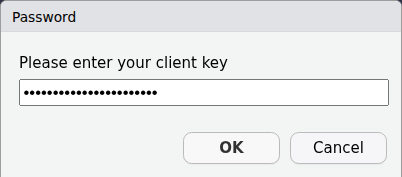
\includegraphics[width=0.6\linewidth,height=\textheight,keepaspectratio]{media/authentication-rstudio.png}

}

\caption{\label{fig-askpass}Screenshot of authentication in the RStudio
IDE}

\end{figure}%

The most useful endpoint that the Research API offers is to search the
platform for posts. For queries, TikTok uses a fine-grained, yet
complicated query syntax.\footnote{See
  \url{https://developers.tiktok.com/doc/research-api-specs-query-videos\#query}.}
For convenience, a query in \texttt{traktok} is constructed internally
when you search with a key phrase directly:

\begin{Shaded}
\begin{Highlighting}[]
\FunctionTok{tt\_query\_videos}\NormalTok{(}\StringTok{"\#rstats"}\NormalTok{, }\AttributeTok{max\_pages =} \DecValTok{2}\NormalTok{L)}
\CommentTok{\#\textgreater{} ── search id: NA ───────────────────────────────────────}
\CommentTok{\#\textgreater{} \# A tibble: 0 × 13}
\CommentTok{\#\textgreater{} \# ℹ 13 variables: video\_id \textless{}lgl\textgreater{}, author\_name \textless{}chr\textgreater{},}
\CommentTok{\#\textgreater{} \#   view\_count \textless{}int\textgreater{}, comment\_count \textless{}int\textgreater{},}
\CommentTok{\#\textgreater{} \#   share\_count \textless{}int\textgreater{}, like\_count \textless{}int\textgreater{},}
\CommentTok{\#\textgreater{} \#   region\_code \textless{}chr\textgreater{}, create\_time \textless{}dttm\textgreater{},}
\CommentTok{\#\textgreater{} \#   effect\_ids \textless{}list\textgreater{}, music\_id \textless{}chr\textgreater{},}
\CommentTok{\#\textgreater{} \#   video\_description \textless{}chr\textgreater{}, hashtag\_names \textless{}list\textgreater{},}
\CommentTok{\#\textgreater{} \#   voice\_to\_text \textless{}chr\textgreater{}}
\end{Highlighting}
\end{Shaded}

This will match a supplied keyword or phrase against keywords and
hashtags and return up to 200 results (each page has 100 results and 2
pages are requested by default) from ten and eleven days ago (the
defaults are \texttt{start\_date\ =\ Sys.Date()\ -\ 11} and
\texttt{end\_date\ =\ Sys.Date()\ -\ 10}). This somewhat odd default
window is deliberate, as TikTok states that new videos take up to 48
hours to be added to the search engine behind the Research API and that
statistics such as the view count can take up to 10 days to
update.\footnote{See
  \url{https://developers.tiktok.com/doc/research-api-faq}.}
Entrena-Serrano et al. (2025) found in their tests that videos were
frequently still missing after 72 hours, so when setting the dates
manually, I recommend leaving a gap of at least three days between the
end date of a query and the day it is run, and of ten days if the
engagement statistics matter for the analysis. Every white-space is
treated as an AND operator. To extend the retrieved range, you can set a
start and end date (there is no limit how far you can go back):

\begin{Shaded}
\begin{Highlighting}[]
\FunctionTok{tt\_query\_videos}\NormalTok{(}\StringTok{"\#rstats"}\NormalTok{,}
                \AttributeTok{max\_pages =} \DecValTok{2}\NormalTok{L,}
                \AttributeTok{start\_date =} \FunctionTok{as.Date}\NormalTok{(}\StringTok{"2023{-}11{-}01"}\NormalTok{),}
                \AttributeTok{end\_date =} \FunctionTok{as.Date}\NormalTok{(}\StringTok{"2023{-}11{-}29"}\NormalTok{))}
\CommentTok{\#\textgreater{} ── search id: 7423432753447932974 ──────────────────────}
\CommentTok{\#\textgreater{} \# A tibble: 19 × 13}
\CommentTok{\#\textgreater{}    video\_id         author\_name view\_count comment\_count}
\CommentTok{\#\textgreater{}    \textless{}chr\textgreater{}            \textless{}chr\textgreater{}            \textless{}int\textgreater{}         \textless{}int\textgreater{}}
\CommentTok{\#\textgreater{}  1 730689385329705… statistics…        909             4}
\CommentTok{\#\textgreater{}  2 730630774458222… learningca…       1104            11}
\CommentTok{\#\textgreater{}  3 730501447636800… picanumeros       4645             8}
\CommentTok{\#\textgreater{}  4 730297066790799… smooth.lea…      98717            17}
\CommentTok{\#\textgreater{}  5 730247037950160… statistics…        508             0}
\CommentTok{\#\textgreater{}  6 730097749816510… statistics…      27387             1}
\CommentTok{\#\textgreater{}  7 730093147605973… rigochando        2603             4}
\CommentTok{\#\textgreater{}  8 730092229522312… elartedeld…        765             0}
\CommentTok{\#\textgreater{}  9 729998705941704… statistics…       1110             1}
\CommentTok{\#\textgreater{} 10 729965751681473… rigochando         905             4}
\CommentTok{\#\textgreater{} 11 729934294487885… rigochando         555             0}
\CommentTok{\#\textgreater{} 12 729896668413454… rigochando        1312             1}
\CommentTok{\#\textgreater{} 13 729691148659145… biofreelan…      19758             7}
\CommentTok{\#\textgreater{} 14 729691148625178… biofreelan…       5763             1}
\CommentTok{\#\textgreater{} 15 729691147878174… biofreelan…       1019             3}
\CommentTok{\#\textgreater{} 16 729668885660947… mrpecners          657             2}
\CommentTok{\#\textgreater{} 17 729651863537426… l\_a\_kelly          514             5}
\CommentTok{\#\textgreater{} 18 729649864535081… mrpecners          373             0}
\CommentTok{\#\textgreater{} 19 729628884337898… casaresfel…        274             0}
\CommentTok{\#\textgreater{} \# ℹ 9 more variables: share\_count \textless{}int\textgreater{},}
\CommentTok{\#\textgreater{} \#   like\_count \textless{}int\textgreater{}, region\_code \textless{}chr\textgreater{},}
\CommentTok{\#\textgreater{} \#   create\_time \textless{}dttm\textgreater{}, effect\_ids \textless{}list\textgreater{},}
\CommentTok{\#\textgreater{} \#   music\_id \textless{}chr\textgreater{}, video\_description \textless{}chr\textgreater{},}
\CommentTok{\#\textgreater{} \#   hashtag\_names \textless{}list\textgreater{}, voice\_to\_text \textless{}chr\textgreater{}}
\end{Highlighting}
\end{Shaded}

The API itself only accepts a start and end that are a maximum of 30
days apart, but \texttt{traktok} takes care of this in the background:
longer time spans are split into consecutive windows of at most 30 days,
which are queried one after the other before the results are combined.
The returned object also carries the start and end date of the last
window as attributes, so that a search can be picked back up where it
stopped more easily.

As said, the query syntax that TikTok uses is a little complicated, as
users can chain queries with \texttt{AND}, \texttt{OR} and \texttt{NOT}
operators (see Table~\ref{tbl-boolean}) on a number of fields
(\texttt{"create\_date"}, \texttt{"username"}, \texttt{"region\_code"},
\texttt{"video\_id"}, \texttt{"hashtag\_name"}, \texttt{"keyword"},
\texttt{"music\_id"}, \texttt{"effect\_id"}, and
\texttt{"video\_length"}).

\begin{longtable}[]{@{}ll@{}}
\caption{Boolean operators as used by
TikTok}\label{tbl-boolean}\tabularnewline
\toprule\noalign{}
Operator & Results are returned if\ldots{} \\
\midrule\noalign{}
\endfirsthead
\toprule\noalign{}
Operator & Results are returned if\ldots{} \\
\midrule\noalign{}
\endhead
\bottomrule\noalign{}
\endlastfoot
AND & \ldots all specified conditions are met \\
OR & \ldots any of the specified conditions are met \\
NOT & \ldots the not conditions are not met \\
\end{longtable}

To make queries easier to use, \texttt{traktok} uses a tidyverse style
approach to building a search. For example, to get to the same query we
used above, which matches \#rstats against keywords and hashtags, you
need to build the query like this:

\begin{Shaded}
\begin{Highlighting}[]
\FunctionTok{query}\NormalTok{() }\SpecialCharTok{|\textgreater{}}                              \CommentTok{\# start by using query()}
  \FunctionTok{query\_or}\NormalTok{(}\AttributeTok{field\_name =} \StringTok{"hashtag\_name"}\NormalTok{, }\CommentTok{\# add an OR condition on the hashtag field}
           \AttributeTok{operation =} \StringTok{"IN"}\NormalTok{,            }\CommentTok{\# the value should be IN the list of hashtags}
           \AttributeTok{field\_values =} \StringTok{"rstats"}\NormalTok{) }\SpecialCharTok{|\textgreater{}}  \CommentTok{\# hashtag field does not accept the \#{-}symbol}
  \FunctionTok{query\_or}\NormalTok{(}\AttributeTok{field\_name =} \StringTok{"keyword"}\NormalTok{,      }\CommentTok{\# add another OR condition}
           \AttributeTok{operation =} \StringTok{"IN"}\NormalTok{,}
           \AttributeTok{field\_values =} \StringTok{"\#rstats"}\NormalTok{)}
\CommentTok{\#\textgreater{} S3\textless{}traktok\_query\textgreater{}}
\CommentTok{\#\textgreater{} └─or: \textless{}list\textgreater{}}
\CommentTok{\#\textgreater{}   ├─\textless{}list\textgreater{}}
\CommentTok{\#\textgreater{}   │ ├─field\_name: "hashtag\_name"}
\CommentTok{\#\textgreater{}   │ ├─operation: "IN"}
\CommentTok{\#\textgreater{}   │ └─field\_values: \textless{}list\textgreater{}}
\CommentTok{\#\textgreater{}   │   └─"rstats"}
\CommentTok{\#\textgreater{}   └─\textless{}list\textgreater{}}
\CommentTok{\#\textgreater{}     ├─field\_name: "keyword"}
\CommentTok{\#\textgreater{}     ├─operation: "IN"}
\CommentTok{\#\textgreater{}     └─field\_values: \textless{}list\textgreater{}}
\CommentTok{\#\textgreater{}       └─"\#rstats"}
\end{Highlighting}
\end{Shaded}

\begin{longtable}[]{@{}ll@{}}
\caption{Condition operators as used by
TikTok}\label{tbl-match}\tabularnewline
\toprule\noalign{}
Operation & Results are returned if field\_values are\ldots{} \\
\midrule\noalign{}
\endfirsthead
\toprule\noalign{}
Operation & Results are returned if field\_values are\ldots{} \\
\midrule\noalign{}
\endhead
\bottomrule\noalign{}
\endlastfoot
EQ & equal to the value in the field \\
IN & equal to a value in the field \\
GT & greater than the value in the field \\
GTE & greater than or equal to the value in the field \\
LT & lower than the value in the field \\
LTE & lower than or equal to the value in the field \\
\end{longtable}

If \#rstats is found in either the hashtag or keywords of a video, that
video is then returned. Besides checking for \texttt{EQ}ual, users can
also use one of the other operations: shown in Table~\ref{tbl-match}.
This makes building queries relatively complex, but allows for
fine-grained searches in the TikTok data:

\begin{Shaded}
\begin{Highlighting}[]
\NormalTok{search\_df }\OtherTok{\textless{}{-}} \FunctionTok{query}\NormalTok{() }\SpecialCharTok{|\textgreater{}}
  \FunctionTok{query\_and}\NormalTok{(}\AttributeTok{field\_name =} \StringTok{"region\_code"}\NormalTok{,}
            \AttributeTok{operation =} \StringTok{"IN"}\NormalTok{,}
            \AttributeTok{field\_values =} \FunctionTok{c}\NormalTok{(}\StringTok{"JP"}\NormalTok{, }\StringTok{"US"}\NormalTok{)) }\SpecialCharTok{|\textgreater{}}
  \FunctionTok{query\_or}\NormalTok{(}\AttributeTok{field\_name =} \StringTok{"hashtag\_name"}\NormalTok{,}
            \AttributeTok{operation =} \StringTok{"EQ"}\NormalTok{, }\CommentTok{\# rstats is the only hashtag}
            \AttributeTok{field\_values =} \StringTok{"rstats"}\NormalTok{) }\SpecialCharTok{|\textgreater{}}
  \FunctionTok{query\_or}\NormalTok{(}\AttributeTok{field\_name =} \StringTok{"keyword"}\NormalTok{,}
           \AttributeTok{operation =} \StringTok{"IN"}\NormalTok{, }\CommentTok{\# rstats is one of the keywords}
           \AttributeTok{field\_values =} \StringTok{"rstats"}\NormalTok{) }\SpecialCharTok{|\textgreater{}}
  \FunctionTok{query\_not}\NormalTok{(}\AttributeTok{operation =} \StringTok{"EQ"}\NormalTok{,}
            \AttributeTok{field\_name =} \StringTok{"video\_length"}\NormalTok{,}
            \AttributeTok{field\_values =} \StringTok{"SHORT"}\NormalTok{) }\SpecialCharTok{|\textgreater{}}
  \FunctionTok{tt\_search\_api}\NormalTok{(}\AttributeTok{start\_date =} \FunctionTok{as.Date}\NormalTok{(}\StringTok{"2023{-}11{-}01"}\NormalTok{),}
                \AttributeTok{end\_date =} \FunctionTok{as.Date}\NormalTok{(}\StringTok{"2023{-}11{-}29"}\NormalTok{))}

\NormalTok{search\_df}
\CommentTok{\#\textgreater{} ── search id: 7423432753447965742 ──────────────────────}
\CommentTok{\#\textgreater{} \# A tibble: 2 × 13}
\CommentTok{\#\textgreater{}   video\_id          author\_name view\_count comment\_count}
\CommentTok{\#\textgreater{}   \textless{}chr\textgreater{}             \textless{}chr\textgreater{}            \textless{}int\textgreater{}         \textless{}int\textgreater{}}
\CommentTok{\#\textgreater{} 1 7296688856609475… mrpecners          657             2}
\CommentTok{\#\textgreater{} 2 7296498645350812… mrpecners          373             0}
\CommentTok{\#\textgreater{} \# ℹ 9 more variables: share\_count \textless{}int\textgreater{},}
\CommentTok{\#\textgreater{} \#   like\_count \textless{}int\textgreater{}, region\_code \textless{}chr\textgreater{},}
\CommentTok{\#\textgreater{} \#   create\_time \textless{}dttm\textgreater{}, effect\_ids \textless{}list\textgreater{},}
\CommentTok{\#\textgreater{} \#   music\_id \textless{}chr\textgreater{}, video\_description \textless{}chr\textgreater{},}
\CommentTok{\#\textgreater{} \#   hashtag\_names \textless{}list\textgreater{}, voice\_to\_text \textless{}chr\textgreater{}}
\end{Highlighting}
\end{Shaded}

This will return videos posted in the US or Japan, that have ``rstats''
as the only hashtag or as one of the keywords and have a length of
\texttt{"MID"}, \texttt{"LONG"}, or \texttt{"EXTRA\_LONG"}.\footnote{
  See
  \url{https://developers.tiktok.com/doc/research-api-specs-query-videos\#condition_fields}
  for possible values of each field.}

Instead of searching for videos by keyword or hashtag, the endpoint also
allows querying all videos a specific account has posted:

\begin{Shaded}
\begin{Highlighting}[]
\FunctionTok{query}\NormalTok{() }\SpecialCharTok{|\textgreater{}}
  \FunctionTok{query\_and}\NormalTok{(}\AttributeTok{field\_name =} \StringTok{"username"}\NormalTok{,}
            \AttributeTok{operation =} \StringTok{"EQ"}\NormalTok{,}
            \AttributeTok{field\_values =} \StringTok{"kamalahq"}\NormalTok{) }\SpecialCharTok{|\textgreater{}}
  \FunctionTok{tt\_search\_api}\NormalTok{(}\AttributeTok{start\_date =} \FunctionTok{as.Date}\NormalTok{(}\StringTok{"2024{-}08{-}01"}\NormalTok{),}
                \AttributeTok{end\_date =} \FunctionTok{as.Date}\NormalTok{(}\StringTok{"2024{-}08{-}31"}\NormalTok{))}

\CommentTok{\#\textgreater{} \# A tibble: 99 × 13}
\CommentTok{\#\textgreater{}    video\_id           author\_name view\_count comment\_count}
\CommentTok{\#\textgreater{}    \textless{}chr\textgreater{}              \textless{}chr\textgreater{}            \textless{}int\textgreater{}         \textless{}int\textgreater{} }
\CommentTok{\#\textgreater{}  1 74093484933299110… kamalahq       1883658          3599 }
\CommentTok{\#\textgreater{}  2 74090413381314347… kamalahq       2485343          1554 }
\CommentTok{\#\textgreater{}  3 74090184761339118… kamalahq        937485          1100}
\CommentTok{\#\textgreater{}  4 74089979841694466… kamalahq       5093111          5693}
\CommentTok{\#\textgreater{}  5 74089584344412029… kamalahq        982621          2075 }
\CommentTok{\#\textgreater{}  6 74089389886664246… kamalahq       3519123          2596}
\CommentTok{\#\textgreater{}  7 74087545861834048… kamalahq        364593           238}
\CommentTok{\#\textgreater{}  8 74087447709082289… kamalahq        831576           869}
\CommentTok{\#\textgreater{}  9 74087072245345190… kamalahq       1257399          3710}
\CommentTok{\#\textgreater{} 10 74086905194395763… kamalahq        408406          1395 }
\CommentTok{\#\textgreater{} \# ℹ 9 more variables: share\_count \textless{}int\textgreater{},}
\CommentTok{\#\textgreater{} \#   like\_count \textless{}int\textgreater{}, region\_code \textless{}chr\textgreater{},}
\CommentTok{\#\textgreater{} \#   create\_time \textless{}dttm\textgreater{}, effect\_ids \textless{}list\textgreater{},}
\CommentTok{\#\textgreater{} \#   music\_id \textless{}chr\textgreater{}, video\_description \textless{}chr\textgreater{},}
\CommentTok{\#\textgreater{} \#   hashtag\_names \textless{}list\textgreater{}, voice\_to\_text \textless{}chr\textgreater{}}
\end{Highlighting}
\end{Shaded}

The second useful function that we are highlighting here is
\texttt{tt\_comments\_api}. Using a video ID, it retrieves the full text
of user comments, along with useful information about the discussion
structure, like and reply counts.

\begin{Shaded}
\begin{Highlighting}[]
\FunctionTok{tt\_comments\_api}\NormalTok{(}\AttributeTok{video\_id =} \StringTok{"7409348493329911082"}\NormalTok{)}

\CommentTok{\#\textgreater{} \# A tibble: 92 × 7}
\CommentTok{\#\textgreater{}    like\_count parent\_comment\_id   reply\_count text    }
\CommentTok{\#\textgreater{}         \textless{}int\textgreater{} \textless{}chr\textgreater{}                     \textless{}int\textgreater{} \textless{}chr\textgreater{}   }
\CommentTok{\#\textgreater{}  1       2302 7409348493329911082          47 I\textquotesingle{}ve ne…}
\CommentTok{\#\textgreater{}  2       2218 7409348493329911082          62 my rank…}
\CommentTok{\#\textgreater{}  3       1865 7409348493329911082          24 My rank…}
\CommentTok{\#\textgreater{}  4        955 7409348493329911082           9 I inten…}
\CommentTok{\#\textgreater{}  5        808 7409348493329911082          12 Don’t t…}
\CommentTok{\#\textgreater{}  6        604 7409348493329911082           5 This ac…}
\CommentTok{\#\textgreater{}  7        421 7409348493329911082          10 Cooked …}
\CommentTok{\#\textgreater{}  8        320 7409348493329911082          15 my team…}
\CommentTok{\#\textgreater{}  9        301 7409348493329911082           4 MADAM P…}
\CommentTok{\#\textgreater{} 10        265 7409348493329911082           5 Assignm…}
\CommentTok{\#\textgreater{} \# ℹ 82 more rows}
\CommentTok{\#\textgreater{} \# ℹ 3 more variables: video\_id \textless{}chr\textgreater{},}
\CommentTok{\#\textgreater{} \#   create\_time \textless{}int\textgreater{}, id \textless{}chr\textgreater{}}
\CommentTok{\#\textgreater{} \# ℹ Use \textasciigrave{}print(n = ...)\textasciigrave{} to see more rows}
\end{Highlighting}
\end{Shaded}

For many research projects, it will also be of value to determine who a
user follows and who they are followed by. This can be accomplished as
shown below:

\begin{Shaded}
\begin{Highlighting}[]
\FunctionTok{tt\_user\_follower\_api}\NormalTok{(}\StringTok{"kamalahq"}\NormalTok{)}
\CommentTok{\#\textgreater{} i Getting user kamalahq}
\CommentTok{\#\textgreater{} v Got user kamalahq [525ms]}
\CommentTok{\#\textgreater{} i Getting user kamalahq}
\CommentTok{\#\textgreater{} \# A tibble: 72 x 3}
\CommentTok{\#\textgreater{}    display\_name   username          following\_user}
\CommentTok{\#\textgreater{}    \textless{}chr\textgreater{}          \textless{}chr\textgreater{}             \textless{}chr\textgreater{}         }
\CommentTok{\#\textgreater{}  1 FroggyFresh    froggyfresh08     kamalahq      }
\CommentTok{\#\textgreater{}  2 Allan          user125137690791  kamalahq      }
\CommentTok{\#\textgreater{}  3 loralorenzo    loralorenzo       kamalahq      }
\CommentTok{\#\textgreater{}  4 aregahengaweke aregahengaweke    kamalahq      }
\CommentTok{\#\textgreater{}  5 Crystal.K      iam\_crystal00     kamalahq      }
\CommentTok{\#\textgreater{}  6 noahtugwo81    noahtugwo81       kamalahq      }
\CommentTok{\#\textgreater{}  7 ree            ree0759           kamalahq      }
\CommentTok{\#\textgreater{}  8 Jim            jimbobaz          kamalahq      }
\CommentTok{\#\textgreater{}  9 ganiyuafeez303 gaotavo007        kamalahq      }
\CommentTok{\#\textgreater{} 10 mosh 2k        user1111552735533 kamalahq      }
\CommentTok{\#\textgreater{} \# i 62 more rows}

\CommentTok{\# kamalahq has set the following information to private, leading to this output}
\FunctionTok{tt\_user\_following\_api}\NormalTok{(}\StringTok{"kamalahq"}\NormalTok{)}
\CommentTok{\#\textgreater{} i Getting user kamalahq}
\CommentTok{\#\textgreater{} x Getting user kamalahq [257ms]}
\CommentTok{\#\textgreater{} ! This information cannot be returned}
\CommentTok{\#\textgreater{} \# A tibble: 0 x 1}
\CommentTok{\#\textgreater{} \# i 1 variable: following\_user \textless{}chr\textgreater{}}
\end{Highlighting}
\end{Shaded}

As Table~\ref{tbl-overview} shows, there are several other functions
that query the Research API, however,
\texttt{tt\_user\_liked\_videos\_api} and
\texttt{tt\_user\_pinned\_videos\_api} query information that is opt-in
and therefore turned off by the large majority of accounts, similar to
the second example above; \texttt{tt\_playlist\_api} relates to a
feature of the platform that is not widely used; and
\texttt{tt\_user\_info\_api} only returns very basic information about
accounts that is usually not meaningful for research.

Importantly, a crucial part of the data, namely the video files
themselves, are not accessible through the Research API --- even though
videos can be downloaded through the official TikTok app. However,
\texttt{traktok} users can instead obtain this data through the `hidden'
API, discussed in the next section.

\section{`Hidden' API}\label{hidden-api}

The unofficial or `hidden' API is essentially what the TikTok website
uses to display you content. How these endpoints work was discovered
through reverse engineering -- that is, studying how the browser
retrieves data to display it and mimicking this behaviour in
\texttt{R}\footnote{The groundwork for this was done by Deen Freelon and
  his pyktok Python package.} -- and TikTok might change how these
endpoints operate at any moment. Nevertheless, the approach has been
working since 2022, with only minor adoptions of the code.

\begin{figure}

\centering{

\pandocbounded{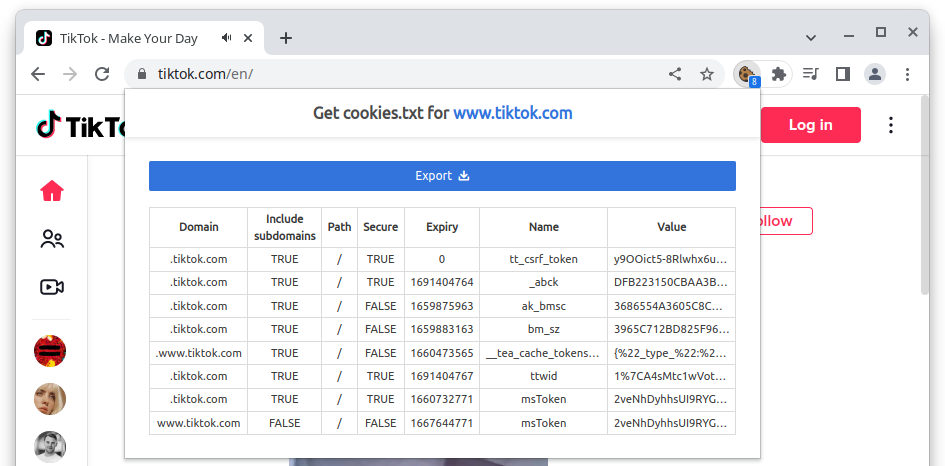
\includegraphics[keepaspectratio]{media/cookies.png}}

}

\caption{\label{fig-cookie}Usage of browser cookies}

\end{figure}%

All functions of the `hidden' API operate by utilizing the cookies
stored in the browser by the website, allowing requests from R to mimic
those from a browser for authentication purposes. HTTP cookies are small
blocks of data websites store in the browser to identify users, which
can range from simple things like remembering your language preference
or items in your shopping cart to more critical functions like keeping
you logged in to your account by storing an authentication token that
verifies your identity with each page you visit. To get these cookies
into \texttt{R}, users can log into their TikTok account (or create a
new one) with a browser on their computer and then use tools like
\href{https://chrome.google.com/webstore/detail/get-cookiestxt-locally/cclelndahbckbenkjhflpdbgdldlbecc}{\emph{Get
cookies.txt}} for Chromium based browsers or
\href{https://addons.mozilla.org/en-US/firefox/addon/cookies-txt/}{\emph{cookies.txt}}
for Firefox\footnote{As almost all browsers used today are based on one
  of these, these two suggestions should satisfy all users.}.
Figure~\ref{fig-cookie} shows how the process works on the browser. It
does not matter if the user downloads all cookies or just the ones
specific to TikTok, as I use the \texttt{cookiemonster} package (Gruber,
2023) to store cookies securely and \texttt{traktok} sends only the
appropriate cookies with its requests. To read the cookies into a
specific encrypted file, a user only has to run the following command
once:

\begin{Shaded}
\begin{Highlighting}[]
\FunctionTok{auth\_hidden}\NormalTok{(}\StringTok{"tiktok.com\_cookies.txt"}\NormalTok{)}
\end{Highlighting}
\end{Shaded}

A few things about these cookies are worth clarifying. A logged in
account is not strictly necessary, as TikTok also sets cookies for
visitors who are not logged in, but the website hides some content, such
as age-restricted videos, from these sessions and prompts a login after
a few dozen search results at most, which is why I recommend logging in
before exporting the cookies. Since the cookies identify the account
uniquely, TikTok could in principle link the requests made by
\texttt{traktok} to it. As of writing, there are no known incidents of
TikTok taking action against the account of a \texttt{traktok} user, but
I still recommend users to rely on throwaway accounts; I return to the
legal side of this in the section on legal and ethical considerations
below.

Like in the Research API, users are able to search for videos, albeit at
a slower pace and only within the range of what would be shown in the
search on the website. Technically, the function opens a browser in the
background and keeps scrolling down until there are no more videos found
or until a predefined end time is reached. One caveat is that TikTok
usually interrupts the scrolling with a CAPTCHA at some point, which is
why the example below sets \texttt{solve\_captchas\ =\ TRUE}; I explain
what happens in that case in the section on combining the APIs below. In
the example below, we search for the hashtag ``rstats'' again and let
the function scroll for two minutes. It is also possible to scroll for
an infinite time, stopping only when no more videos are returned.
However, whether or not an end time is defined, the user can always
cancel the process without loosing data. After the function stopped or
was stopped, the previous search can still be retrieved with
\texttt{last\_query()}.

\begin{Shaded}
\begin{Highlighting}[]
\FunctionTok{library}\NormalTok{(traktok)}
\NormalTok{rstats\_df\_f }\OtherTok{\textless{}{-}} \StringTok{"rstats\_df.rds"}
\ControlFlowTok{if}\NormalTok{ (}\SpecialCharTok{!}\FunctionTok{file.exists}\NormalTok{(rstats\_df\_f)) \{}
\NormalTok{  rstats\_urls }\OtherTok{\textless{}{-}} \FunctionTok{tt\_search\_hidden}\NormalTok{(}
    \StringTok{"\#rstats"}\NormalTok{,}
    \AttributeTok{scroll =} \StringTok{"2minutes"}\NormalTok{,}
    \AttributeTok{solve\_captchas =} \ConstantTok{TRUE}
\NormalTok{  )}
  \FunctionTok{saveRDS}\NormalTok{(rstats\_urls, rstats\_df\_f)}
\NormalTok{\}}
\NormalTok{rstats\_urls }\OtherTok{\textless{}{-}} \FunctionTok{readRDS}\NormalTok{(rstats\_df\_f)}
\NormalTok{rstats\_urls}
\end{Highlighting}
\end{Shaded}

\begin{Shaded}
\begin{Highlighting}[]
\CommentTok{\#| eval: false}
\NormalTok{rstats\_urls }\OtherTok{\textless{}{-}} \FunctionTok{tt\_search\_hidden}\NormalTok{(}
    \StringTok{"\#rstats"}\NormalTok{,}
    \AttributeTok{scroll =} \StringTok{"2minutes"}\NormalTok{,       }\CommentTok{\# stop scrolling after 2 minutes}
    \AttributeTok{solve\_captchas =} \ConstantTok{TRUE}      \CommentTok{\# open a browser window if a captcha is detected}
\NormalTok{  )}
\FunctionTok{head}\NormalTok{(rstats\_urls)}
\CommentTok{\#\textgreater{}  [1] "https://www.tiktok.com/@statisticsglobe/video/7252226153828584731"     }
\CommentTok{\#\textgreater{}  [2] "https://www.tiktok.com/@learningcast/video/7212048931172306222"        }
\CommentTok{\#\textgreater{}  [3] "https://www.tiktok.com/@plantitareal/video/7171033929175026949"        }
\CommentTok{\#\textgreater{}  [4] "https://www.tiktok.com/@learningcast/video/7247854060500421934"        }
\CommentTok{\#\textgreater{}  [5] "https://www.tiktok.com/@statisticsglobe/video/7237474759536135430"     }
\CommentTok{\#\textgreater{}  [6] "https://www.tiktok.com/@mrpecners/video/7274045053889285419"}
\FunctionTok{head}\NormalTok{(}\FunctionTok{last\_query}\NormalTok{())}
\CommentTok{\#\textgreater{}  [1] "https://www.tiktok.com/@statisticsglobe/video/7252226153828584731"     }
\CommentTok{\#\textgreater{}  [2] "https://www.tiktok.com/@learningcast/video/7212048931172306222"        }
\CommentTok{\#\textgreater{}  [3] "https://www.tiktok.com/@plantitareal/video/7171033929175026949"        }
\CommentTok{\#\textgreater{}  [4] "https://www.tiktok.com/@learningcast/video/7247854060500421934"        }
\CommentTok{\#\textgreater{}  [5] "https://www.tiktok.com/@statisticsglobe/video/7237474759536135430"     }
\CommentTok{\#\textgreater{}  [6] "https://www.tiktok.com/@mrpecners/video/7274045053889285419"   }
\end{Highlighting}
\end{Shaded}

Additionally, we can query all videos posted by a specific user account.
The first step to take this is to find out the internal ID of a user:

\begin{Shaded}
\begin{Highlighting}[]
\NormalTok{kamalahq\_info }\OtherTok{\textless{}{-}} \FunctionTok{tt\_user\_info\_hidden}\NormalTok{(}\StringTok{"kamalahq"}\NormalTok{)}
\end{Highlighting}
\end{Shaded}

The important piece of information is stored in the column
\texttt{secUid}, which we can hand to the
\texttt{tt\_get\_follower\_hidden} function:

\begin{Shaded}
\begin{Highlighting}[]
\NormalTok{kamalahq\_follower }\OtherTok{\textless{}{-}} \FunctionTok{tt\_get\_follower\_hidden}\NormalTok{(kamalahq\_info}\SpecialCharTok{$}\NormalTok{secUid)}
\FunctionTok{nrow}\NormalTok{(kamalahq\_following)}
\CommentTok{\#\textgreater{} 4881}
\end{Highlighting}
\end{Shaded}

This does not deliver the full set of followers, but only returns what
would be visible on the web version. It additionally takes much longer
than the Research API version. Therefore, running the function is only
interesting for researcher who do no have access to the official API.

The most important feature of the `hidden' API, however, which is
interesting also for users who already have access to the Research API,
is to query information about specific posts and being able to download
the videos or images included in them. This is implemented in the
\texttt{tt\_videos} function:

\begin{Shaded}
\begin{Highlighting}[]
\CommentTok{\# this comes from a previously saved search}
\NormalTok{rstats\_df  }\OtherTok{\textless{}{-}} \FunctionTok{readRDS}\NormalTok{(}\StringTok{"search\_results.rds"}\NormalTok{)}
\NormalTok{rstats\_df2 }\OtherTok{\textless{}{-}} \FunctionTok{tt\_videos}\NormalTok{(rstats\_df}\SpecialCharTok{$}\NormalTok{video\_url[}\DecValTok{1}\SpecialCharTok{:}\DecValTok{2}\NormalTok{], }\AttributeTok{save\_video =} \ConstantTok{TRUE}\NormalTok{)}

\NormalTok{rstats\_df2}
\CommentTok{\#\textgreater{} \# A tibble: 2 × 25}
\CommentTok{\#\textgreater{}   video\_id   video\_url video\_timestamp     video\_length video\_title}
\CommentTok{\#\textgreater{}   \textless{}glue\textgreater{}     \textless{}chr\textgreater{}     \textless{}dttm\textgreater{}                     \textless{}int\textgreater{} \textless{}chr\textgreater{}      }
\CommentTok{\#\textgreater{} 1 711511441… https://… 2022{-}06{-}30 19:17:53          135 R for Begi…}
\CommentTok{\#\textgreater{} 2 725222615… https://… 2023{-}07{-}05 07:01:45           36 Wow!!! THI…}
\CommentTok{\#\textgreater{} \# ℹ 20 more variables: video\_locationcreated \textless{}chr\textgreater{},}
\CommentTok{\#\textgreater{} \#   video\_diggcount \textless{}int\textgreater{}, video\_sharecount \textless{}int\textgreater{},}
\CommentTok{\#\textgreater{} \#   video\_commentcount \textless{}int\textgreater{}, video\_playcount \textless{}int\textgreater{},}
\CommentTok{\#\textgreater{} \#   author\_id \textless{}chr\textgreater{}, author\_secuid \textless{}chr\textgreater{}, author\_username \textless{}chr\textgreater{},}
\CommentTok{\#\textgreater{} \#   author\_nickname \textless{}chr\textgreater{}, author\_bio \textless{}chr\textgreater{}, download\_url \textless{}chr\textgreater{},}
\CommentTok{\#\textgreater{} \#   html\_status \textless{}int\textgreater{}, music \textless{}list\textgreater{}, challenges \textless{}list\textgreater{},}
\CommentTok{\#\textgreater{} \#   is\_secret \textless{}lgl\textgreater{}, is\_for\_friend \textless{}lgl\textgreater{}, is\_slides \textless{}lgl\textgreater{}, …}
\end{Highlighting}
\end{Shaded}

When users are scraping many URLs, which in my experience means
thousands rather than hundreds, the function often fails eventually for
one reason or another. It therefore usually makes sense to save progress
in a cache directory:

\begin{Shaded}
\begin{Highlighting}[]
\NormalTok{rstats\_df3 }\OtherTok{\textless{}{-}} \FunctionTok{tt\_videos}\NormalTok{(rstats\_df}\SpecialCharTok{$}\NormalTok{video\_url[}\DecValTok{5}\SpecialCharTok{:}\DecValTok{6}\NormalTok{], }\AttributeTok{cache\_dir =} \StringTok{"rstats"}\NormalTok{)}

\FunctionTok{list.files}\NormalTok{(}\StringTok{"rstats"}\NormalTok{)}
\CommentTok{\#\textgreater{} [1] "7257689890245201153.json" "7299987059417042209.json"}
\end{Highlighting}
\end{Shaded}

With this, the package comfortably handles the scale of most research
projects, which I would put at somewhere between a handful and around a
hundred thousand videos. I have tested the functions with collections of
about twenty thousand videos, which takes some time, and larger
collections are possible with patience, but industrial-scale scraping of
the platform is not what \texttt{traktok} is intended for.

Note that the video files are downloaded into your working directory by
default\footnote{Can be controlled with the \texttt{dir} argument in
  \texttt{tt\_videos}.}, independently of the cache directory.
\texttt{tt\_videos} already retrieves some information that is otherwise
not available, like the video\_status, which shows a reason when a video
is no longer available. If there are information that users feel are
missing from the \texttt{data.frame} that \texttt{tt\_videos} returns,
they can also access the raw, unparsed json data using:

\begin{Shaded}
\begin{Highlighting}[]
\NormalTok{rstats\_list1 }\OtherTok{\textless{}{-}} \FunctionTok{tt\_request\_hidden}\NormalTok{(rstats\_df}\SpecialCharTok{$}\NormalTok{video\_url[}\DecValTok{1}\NormalTok{]) }\SpecialCharTok{|\textgreater{}}
\NormalTok{  jsonlite}\SpecialCharTok{::}\FunctionTok{fromJSON}\NormalTok{()}
\end{Highlighting}
\end{Shaded}

Parsing the result into a list using \texttt{fromJSON}, results in a
complex nested list, which users can explore further. At the time of
writing, this list contains, for example, the text of stickers placed on
the video, an indicator whether the post is an advertisement, links to
automatically generated subtitles, the follower count of the author and
a label for AI-generated content, none of which are part of the parsed
\texttt{data.frame} yet. These fields are candidates to be added to the
output of \texttt{tt\_videos} in upcoming versions, as I extend the
parser whenever fields turn out to be useful for research. I refrain
from documenting the raw data in more detail, however, as TikTok keeps
changing which fields are available.

\section{Combining the APIs}\label{combining-the-apis}

As the TikTok Research API does not deliver video or image files, any
analysis of the content of posts prerequisites an alternative route to
accessing these data. \texttt{traktok} enables this access via the
function \texttt{tt\_videos\_hidden}. As an example for combining both
APIs, let's say we want to acquire all posts from ``kamalahq'', the
campaign account of US presidential election candidate Kamala Harris,
from August 2024. We can first search for post URLs using the Research
API:

\begin{Shaded}
\begin{Highlighting}[]
\NormalTok{kamalahq\_df }\OtherTok{\textless{}{-}} \FunctionTok{query}\NormalTok{() }\SpecialCharTok{|\textgreater{}}
  \FunctionTok{query\_and}\NormalTok{(}\AttributeTok{field\_name =} \StringTok{"username"}\NormalTok{,}
            \AttributeTok{operation =} \StringTok{"EQ"}\NormalTok{,}
            \AttributeTok{field\_values =} \StringTok{"kamalahq"}\NormalTok{) }\SpecialCharTok{|\textgreater{}}
  \FunctionTok{tt\_search\_api}\NormalTok{(}\AttributeTok{start\_date =} \FunctionTok{as.Date}\NormalTok{(}\StringTok{"2024{-}08{-}01"}\NormalTok{),}
                \AttributeTok{end\_date =} \FunctionTok{as.Date}\NormalTok{(}\StringTok{"2024{-}08{-}31"}\NormalTok{))}
\end{Highlighting}
\end{Shaded}

And then download the video and image files through
\texttt{tt\_videos\_hidden}:

\begin{Shaded}
\begin{Highlighting}[]

\NormalTok{results\_df }\OtherTok{\textless{}{-}} \FunctionTok{tt\_videos\_hidden}\NormalTok{(kamalahq\_df}\SpecialCharTok{$}\NormalTok{video\_id,}
                               \AttributeTok{save\_video =} \ConstantTok{TRUE}\NormalTok{,}
                               \AttributeTok{cache\_dir =} \StringTok{"kamalahq"}\NormalTok{,}
                               \AttributeTok{dir =} \StringTok{"kamalahq"}\NormalTok{, }
                               \AttributeTok{slideshows =} \ConstantTok{TRUE}\NormalTok{)}

\FunctionTok{list.files}\NormalTok{(}\StringTok{"kamalahq"}\NormalTok{) }\SpecialCharTok{|\textgreater{}} 
\NormalTok{  tools}\SpecialCharTok{::}\FunctionTok{file\_ext}\NormalTok{() }\SpecialCharTok{|\textgreater{}} 
  \FunctionTok{table}\NormalTok{()}
\CommentTok{\#\textgreater{} jpeg json  mp4 }
\CommentTok{\#\textgreater{}   96   99   70 }
\end{Highlighting}
\end{Shaded}

As can be seen, the function downloaded 70 video files and additionally
96 image files, which are now also often shared on the platform, copying
one of Instagram's main features. These image files belong to so-called
slideshows or photo posts, for which TikTok has recently stopped
including the data in the page source that \texttt{tt\_videos\_hidden}
reads. \texttt{traktok} therefore recognises slideshows among the URLs
and, once all other posts are collected, asks whether to hand them to
\texttt{tt\_slideshow\_hidden} (or does so directly with
\texttt{slideshows\ =\ TRUE}), which opens each post in a browser in the
background, waits until the site has requested the post data itself and
collects the metadata and images from there. As the audio track is often
as important for understanding these posts as the images, the function
also downloads the music of a slideshow as an mp3 file next to the
images. Since the cache was set to the same folder, we also get the raw
data as json files. This has the side effect that already downloaded
data is not requested again, if we rerun the function, for example, with
an extended list of video IDs.

The second important use case for combining both APIs is to compare them
to assess the completeness of results, as has been done for Facebook
(Ho, 2020) and Twitter (Tromble et al., 2017) in the past. As mentioned
in the introduction, Germany's far right party AFD has managed to build
a hard to overlook presence on TikTok, and serves as a demonstration
case here. For convenience, \texttt{traktok} provides the function
\texttt{tt\_user\_videos\_api}, which makes queries to the Research API
for all videos a user has published:

\begin{Shaded}
\begin{Highlighting}[]
\NormalTok{results\_api }\OtherTok{\textless{}{-}} \FunctionTok{tt\_user\_videos\_api}\NormalTok{(}
  \AttributeTok{username =} \StringTok{"afdfraktionimbundestag"}\NormalTok{,}
  \AttributeTok{since =} \StringTok{"2020{-}01{-}01"}
\NormalTok{)}
\end{Highlighting}
\end{Shaded}

The same function also exists for the `hidden' API:

\begin{Shaded}
\begin{Highlighting}[]
\NormalTok{results\_scraping }\OtherTok{\textless{}{-}} \FunctionTok{tt\_user\_videos\_hidden}\NormalTok{(}
  \AttributeTok{username =} \StringTok{"afdfraktionimbundestag"}\NormalTok{,}
  \AttributeTok{solve\_captchas =} \ConstantTok{TRUE}
\NormalTok{)}
\end{Highlighting}
\end{Shaded}

This will open a real browser in the background that scrolls down on a
specific account site until the beginning of a user's timeline is
reached. This process will often trigger so-called \emph{CAPTCHA}s,
which are small challenges created to test if a human or bot is
performing an action on the site. If that happens, and the argument
\texttt{solve\_captchas} is true, the browser will jump to the
foreground, so that a user can solve it and \texttt{traktok} can
continue scrolling.

Comparing the results from the Research API and the scraping effort, we
see some discrepancies. The Research API delivered 308, while the
`hidden' API found 319 posts. However, the content is also not as
similar as these numbers suggest. 15 posts were only accessible via the
website, while 4 posts were found by the API, but not actually present
on the website. Searching manually for the videos not present on the
channel page on the website, it turns out that these videos were
restricted by TikTok as they contain extreme or age-restricted content
-- which can also be obtained through the Hidden API by logging in as an
age-verified user. We currently do not know why the search from the API
is incomplete (I come back to this in the final section).

\section{Legal and ethical
considerations}\label{legal-and-ethical-considerations}

Studying TikTok comes with some important legal and ethical
considerations, which researchers should keep in mind. First, when
collecting data via APIs or web scraping, researchers must navigate data
privacy regulations, particularly the General Data Protection Regulation
(GDPR) in Europe and similar frameworks globally which protect personal
data of users (European Union, 2016). As posts on TikTok often contain
such personal data, \texttt{traktok} users usually need to familiarize
themselves with what they can and cannot do with the data they obtain.
One option to legally acquire and share the data would be to obtain
informed consent from the persons who appear in posts (Breuer et al.,
2025). Yet, collecting public data in bulk makes individual consent
impractical (Ohme et al., 2024). There are certain exceptions for
research on systemic risks, which mandate additional requirements for
the research pipeline, especially data minimization principles though
--- that is, collecting only data necessary for addressing specific
research questions (Breuer et al., 2025). Preprocessing steps to remove
personally identifiable information before analysis are essential (Ohme
et al., 2024), though even seemingly anonymous data like follower counts
with timestamps can enable re-identification (Williams et al., 2017).
For \texttt{traktok} users, this means deciding before the collection
which of the returned fields a research question actually requires and
discarding the rest: the \texttt{data.frame} returned by
\texttt{tt\_videos}, for instance, contains the usernames, display names
and biographies of authors, which many analyses do not need, and the
cache directory and the downloaded video files contain the complete,
unprocessed data, which should be stored securely and deleted once they
have served their purpose.

Secondly, platform-centric methods like scraping public content operate
in a legally ambiguous space: while cases like HiQ v. LinkedIn in the
United States have upheld the legality of scraping publicly accessible
data without breaching technological barriers (German Data Forum
(RatSWD), 2020), researchers must still try to respect platform Terms of
Service and consider that users may not be aware their public data can
be used for research (Breuer et al., 2025). The two ways of accessing
TikTok described above differ in this respect: the Research API is an
official channel, whose terms researchers accept when they apply for
access, whereas the `hidden' API needs to be considered scraping, and
TikTok's Terms of Service prohibit extracting data from the platform
with automated software that TikTok has not approved.\footnote{See the
  section ``What you can't do on the Platform'' in the terms for the
  European Economic Area,
  \url{https://www.tiktok.com/legal/page/eea/terms-of-service/en}; the
  terms for the United States,
  \url{https://www.tiktok.com/legal/page/us/terms-of-service/en},
  contain the same clause.}

Brown et al. (2025) review the case law for the United States and
conclude that the legal risk is lowest when researchers collect only
what is publicly accessible without an account and do not circumvent
technical barriers, and that it is higher when data are collected
through an account, as the `hidden' API functions of \texttt{traktok}
can do, since the account holder has agreed to the terms and the
platform can withdraw its permission at any time, for example by
blocking the account. A breach of the Terms of Service alone is not a
criminal offence in the United States and the platform would have to
demonstrate actual harm, which is difficult in the case of
non-commercial research (Brown et al., 2025), but even though unlikely,
legal dispute is costly and, as Brown et al. (2025) point out, a
university's legal department represents the university rather than the
individual researcher.

I therefore recommend that users consult their institution's legal
counsel and data protection officer before collecting data at scale with
the `hidden' API, and clarify at the same time whether the institution
would support them should TikTok take action against them. Zero legal
risk is not attainable in this area, and excessive caution comes at the
cost of research that is in the public interest (Brown et al., 2025),
which is why \texttt{traktok} is built to stay within what a regular
user could do in a browser: the functions of the `hidden' API wait a
random interval between requests (see the \texttt{sleep\_pool}
argument), which keeps the pace of requests, and thereby the load on
TikTok's servers, close to that of a human user, and when the site asks
for a CAPTCHA, the browser is handed to the user rather than the
challenge being circumvented.

Thirdly, the Digital Services Act (DSA) in the European Union introduces
new provisions mandating platforms to provide data access to qualified
researchers (Ausloos \& Veale, 2021), potentially reducing dependency on
platform cooperation and legally and ethically ambiguous data collection
methods. However, implementation details and enforcement mechanisms
remain evolving. Finally, researchers should consider the ethical
implications of studying vulnerable populations, particularly given
TikTok's young user base, and the potential harms from analyzing
sensitive content without appropriate safeguards (Breuer et al., 2025).
Questions like these are what institutional ethics boards are for, and I
recommend involving them early, before a collection has started, rather
than after the fact (Brown et al., 2025).

\section{Current status and future}\label{current-status-and-future}

\texttt{traktok} provides access to TikTok, a social media platform of
growing societal importance, that should be systematically studied by
communication researchers. While it is not the first or only tool to do
so, the combination of access through the Research API and web scraping
methods in one \texttt{R} package with an easy-to-understand consistent
syntax is built to encourage this research.

Several studies have used the package already to make important
contributions. In communication research, Wirz et al. (2023) studied the
posts of news organizations on TikTok compared with the same outlets'
websites and found a high quality of news report, though be it with more
focus on emotional and soft news. Similarly, Wirz \& Zai (2025) studied
Instagram and TikTok content by news companies, finding that many
outlets still share high quality news content, peppered with some more
entertainment. Hohner et al. (2024) studied mobilization strategies of
far-right groups on TikTok and found distinct communication strategies
like using conspiracy narratives and anti-elitism. Widholm et al. (2024)
studied election campaign videos in Sweden, revealing that youth
organizations had the most prominent accounts and that right-wing
content resulted in more engagement. Peterson-Salahuddin (2025) found
that the ``TikTok's predominantly Gen-Z users engage the platform to
discuss, negotiate, and put in place socially progressive norms around
racism, sexism, and homophobia'' (p.~430).

But also beyond communication research, the package has already been
employed for important contributions. In medicine, Blakeman et al.
(2025) studied posts with health-related information on Twitter (X),
Instagram, and, using \texttt{traktok} also TikTok. Donaldson et al.
(2025) studied how especially young users discuss nicotine pouches on
TikTok, with the result that many videos featured pro-tobacco themes.

The discrepancy between the Research API and the website that I showed
in the section on combining the APIs also deserves a closer look, as it
is not a quirk of my example but has by now been confirmed at a larger
scale. Pearson et al. (2025) audited the API against the website and
likewise found publicly available videos that the API did not return,
along with view counts that were, for data collected before July 2024,
orders of magnitude lower than those displayed on the website and errors
when filtering by username; Corso et al. (2024) obtained at most 65\% of
the videos they requested when drawing a random sample over six years;
and Entrena-Serrano et al. (2025) found that one in eight videos in a
donated dataset of around 260,000 posts were publicly available on the
website but not retrievable through the API. TikTok has not explained
these gaps, but the audits allow for informed assumptions: besides
deleted and private videos, which the documentation mentions, the API
withholds advertisements, videos posted by TikTok itself, everything by
creators it locates in Canada and, for no apparent reason, some accounts
altogether, while a share of the missing videos remains unexplained
(Entrena-Serrano et al., 2025). For researchers this means that the
Research API should not be mistaken for a complete record and that
scraping the website remains the only way to check what it delivers,
which is a second reason for keeping both routes in one package.

As noted above, TikTok can change the endpoints behind the `hidden' API
at any time, and there is no guarantee that the Research API stays as it
is either. I therefore intend to keep maintaining \texttt{traktok} for
the foreseeable future: development happens openly in the GitHub
repository\footnote{\url{https://anonymous.4open.science/r/traktok-26DD}},
where users can report problems and contribute fixes, and stable
versions are published on CRAN (the Comprehensive R Archive Network).
Should I at some point be unable to continue this work, which I consider
unlikely, I will look for a successor and hand the package over to a new
maintainer or organization rather than let it go stale.

\newpage

\section*{References}\label{references}
\addcontentsline{toc}{section}{References}

\protect\phantomsection\label{refs}
\begin{CSLReferences}{1}{0}
\bibitem[\citeproctext]{ref-ausloos_researching_2021}
Ausloos, J., \& Veale, M. (2021). Researching with {Data} {Rights}.
\emph{Technology and Regulation}, \emph{2020}, 136--157.
\url{https://doi.org/10.71265/sfcgjr17}

\bibitem[\citeproctext]{ref-bauer_beauty_2024}
Bauer, M. F. (2024). Beauty, baby and backlash? {Anti}-feminist
influencers on {TikTok}. \emph{Feminist Media Studies}, \emph{24}(5),
1023--1041. \url{https://doi.org/10.1080/14680777.2023.2263820}

\bibitem[\citeproctext]{ref-blakeman_describing_2025}
Blakeman, J. R., Carpenter, N., \& Calderon, S. J. (2025). Describing
acute coronary syndrome symptom information on social media platforms.
\emph{Heart \& Lung}, \emph{70}, 112--121.
\url{https://doi.org/10.1016/j.hrtlng.2024.11.021}

\bibitem[\citeproctext]{ref-boeker_empirical_2022}
Boeker, M., \& Urman, A. (2022). An {Empirical} {Investigation} of
{Personalization} {Factors} on {TikTok}. \emph{Proceedings of the {ACM}
{Web} {Conference} 2022, {WWW} '22}, 2298--2309.
\url{https://doi.org/10.1145/3485447.3512102}

\bibitem[\citeproctext]{ref-breuer_overview_2025}
Breuer, J., Stier, S., Lukito, J., Mangold, F., Wieland, M., \&
Radovanović, D. (2025). \emph{Overview of {Ethical} {Considerations}
when {Working} with {Digital} {Behavioral} {Data} ({GESIS} {Guides} to
{Digital} {Behavioral} {Data}, 14)}. GESIS - Leibniz-Institute for the
Social Sciences. \url{https://doi.org/10.60762/GGDBD25014.1.0}

\bibitem[\citeproctext]{ref-brown_web_2025}
Brown, M. A., Gruen, A., Maldoff, G., Messing, S., Sanderson, Z., \&
Zimmer, M. (2025). Web scraping for research: {Legal}, ethical,
institutional, and scientific considerations. \emph{Big Data \&
Society}, \emph{12}(4), 20539517251381686.
\url{https://doi.org/10.1177/20539517251381686}

\bibitem[\citeproctext]{ref-cervi_tiktok_2023}
Cervi, L., Tejedor, S., \& Blesa, F. G. (2023). {TikTok} and {Political}
{Communication}: {The} {Latest} {Frontier} of {Politainment}? {A} {Case}
{Study}. \emph{Media and Communication}, \emph{11}(2).
\url{https://doi.org/10.17645/mac.v11i2.6390}

\bibitem[\citeproctext]{ref-corso_what_2024}
Corso, F., Pierri, F., \& De Francisci Morales, G. (2024). What we can
learn from {TikTok} through its {Research} {API}. \emph{Companion
{Proceedings} of the 16th {ACM} {Web} {Science} {Conference}}, 110--114.
\url{https://doi.org/10.1145/3630744.3663611}

\bibitem[\citeproctext]{ref-cran}
CRAN. (2025). \emph{The comprehensive r archive network}. R Foundation
for Statistical Computing. \url{https://CRAN.R-project.org/}

\bibitem[\citeproctext]{ref-dhoest_manosphere_2025}
Dhoest, A. (2025). From {Manosphere} to {Mainstream}: {Representations}
of {Masculinity} on {TikTok}. \emph{International Journal of
Communication}, \emph{19}, 20--20.
\url{https://ijoc.org/index.php/ijoc/article/view/24706}

\bibitem[\citeproctext]{ref-donaldson_describing_2025}
Donaldson, S. I., La Capria, K., DeJesus, A., Ganz, O., Delnevo, C. D.,
\& Allem, J.-P. (2025). Describing {ZYN}-{Related} {Content} on
{TikTok}: {Content} {Analysis}. \emph{Nicotine and Tobacco Research},
ntaf016. \url{https://doi.org/10.1093/ntr/ntaf016}

\bibitem[\citeproctext]{ref-egan_reuters_2026}
Egan, J., Robertson, C. T., Ross Arguedas, A., Newman, N., Nielsen, R.
K., Mukherjee, M., \& Fletcher, R. (2026). \emph{Reuters {Institute}
{Digital} {News} {Report} 2026}. Reuters Institute for the Study of
Journalism. \url{https://doi.org/10.60625/risj-4vgf-s811}

\bibitem[\citeproctext]{ref-entrena-serrano_tiktoks_2025}
Entrena-Serrano, C., Degeling, M., Romano, S., \& Çetin, R. B. (2025).
\emph{{TikTok}'s {Research} {API}: {Problems} {Without} {Explanations}}.
arXiv. \url{https://doi.org/10.48550/arXiv.2506.09746}

\bibitem[\citeproctext]{ref-european_union_regulation_2016}
European Union. (2016). Regulation ({EU}) 2016/679 of the {European}
{Parliament} and of the {Council} of 27 {April} 2016 on the protection
of natural persons with regard to the processing of personal data and on
the free movement of such data, and repealing {Directive} 95/46/{EC}
({General} {Data} {Protection} {Regulation}). In \emph{Official Journal
of the European Union} (pp. 1--88).
\url{https://eur-lex.europa.eu/eli/reg/2016/679/oj}

\bibitem[\citeproctext]{ref-ratswd_big_2020}
German Data Forum (RatSWD). (2020). Big data in social, behavioural, and
economic sciences: {Data} access and research data management. In
\emph{RatSWD Output Paper Series}.
\url{https://doi.org/10.17620/02671.52}

\bibitem[\citeproctext]{ref-cookiemonster}
Gruber, J. B. (2023). \emph{{cookiemonster}: Your friendly solution to
managing browser cookies in {R}}.
\url{https://github.com/JBGruber/cookiemonster}

\bibitem[\citeproctext]{ref-guinaudeau_fifteen_2022}
Guinaudeau, B., Munger, K., \& Votta, F. (2022). Fifteen {Seconds} of
{Fame}: {TikTok} and the {Supply} {Side} of {Social} {Video}.
\emph{Computational Communication Research}, \emph{4}(2), 463--485.
\url{https://doi.org/10.5117/ccr2022.2.004.guin}

\bibitem[\citeproctext]{ref-hofacebook2020}
Ho, J. C.-T. (2020). How biased is the sample? {Reverse} engineering the
ranking algorithm of {Facebook}'s {Graph} application programming
interface. \emph{Big Data \& Society}, \emph{7}(1), 2053951720905874.
\url{https://doi.org/10.1177/2053951720905874}

\bibitem[\citeproctext]{ref-hohner_analysing_2024}
Hohner, J., Kakavand, A. E., \& Rothut, S. (2024). Analyzing radical
visuals at scale: {How} far-right groups mobilize on {TikTok}.
\emph{Journal of Digital Social Research}, \emph{6}(1).
\url{https://doi.org/10.33621/jdsr.v6i1.200}

\bibitem[\citeproctext]{ref-kim_going_2023}
Kim, S. J., Villanueva, I. I., \& Chen, K. (2023). Going {Beyond}
{Affective} {Polarization}: {How} {Emotions} and {Identities} are {Used}
in {Anti}-{Vaccination} {TikTok} {Videos}. \emph{Political
Communication}, \emph{41}(4), 588--607.
\url{https://doi.org/10.1080/10584609.2023.2243852}

\bibitem[\citeproctext]{ref-medina_serrano_dancing_2020}
Medina Serrano, J. C., Papakyriakopoulos, O., \& Hegelich, S. (2020).
Dancing to the {Partisan} {Beat}: {A} {First} {Analysis} of {Political}
{Communication} on {TikTok}. \emph{12th {ACM} {Conference} on {Web}
{Science}}, 257--266. \url{https://doi.org/10.1145/3394231.3397916}

\bibitem[\citeproctext]{ref-munger_thirst_2025}
Munger, K., \& Li, V. (2025). Thirst {Traps} and {Quick} {Cuts}: {The}
{Effects} of {TikTok} {``{Edits}''} on {Evaluations} of {Politicians}.
\emph{Social Media + Society}, \emph{11}(2), 20563051251329990.
\url{https://doi.org/10.1177/20563051251329990}

\bibitem[\citeproctext]{ref-newman_reuters_2023}
Newman, N., Fletcher, R., Eddy, K., Robertson, C. T., \& Nielsen, R. K.
(2023). \emph{Reuters {Institute} {Digital} {News} {Report} 2023}.
Reuters Institute for the Study of Journalism.
\url{https://doi.org/10.60625/risj-p6es-hb13}

\bibitem[\citeproctext]{ref-ohme_digital_2024}
Ohme, J., Araujo, T., Boeschoten, L., Freelon, D., Ram, N., Reeves, B.
B., \& Robinson, T. N. (2024). Digital {Trace} {Data} {Collection} for
{Social} {Media} {Effects} {Research}: {APIs}, {Data} {Donation}, and
({Screen}) {Tracking}. \emph{Communication Methods and Measures},
\emph{18}(2), 124--141.
\url{https://doi.org/10.1080/19312458.2023.2181319}

\bibitem[\citeproctext]{ref-askpass}
Ooms, J. (2024). \emph{Askpass: Password entry utilities for r, git, and
SSH}. \url{https://CRAN.R-project.org/package=askpass}

\bibitem[\citeproctext]{ref-pearson_tiktok_api_2025}
Pearson, G. D. H., Silver, N. A., Robinson, J. Y., Azadi, M., Schillo,
B. A., \& Kreslake, J. M. (2025). Beyond the margin of error: A
systematic and replicable audit of the {TikTok} research {API}.
\emph{Information, Communication \& Society}, \emph{28}(3), 452--470.
\url{https://doi.org/10.1080/1369118x.2024.2420032}

\bibitem[\citeproctext]{ref-peterson-salahuddin_teachable_2025}
Peterson-Salahuddin, C. (2025). Teachable moments: {TikTok} social drama
as a site of {Black} feminist intellectual production.
\emph{Information, Communication \& Society}, \emph{28}(3), 417--434.
\url{https://doi.org/10.1080/1369118X.2024.2388093}

\bibitem[\citeproctext]{ref-tjaden_does_2025}
Tjaden, J., Wolfgram, J., Philipp, A., Weißmann, S., Bobzien, L.,
Kohler, U., \& Verwiebe, R. (2025). \emph{Does the {TikTok} feed lean
right? {Exposure} to {Political} {Party} {Content} among non-partisan
users during regional and federal elections in {Germany}}.
\url{https://doi.org/10.31235/osf.io/7vdex_v1}

\bibitem[\citeproctext]{ref-tromble_twitter_2017}
Tromble, R., Storz, A., \& Stockmann, D. (2017). We {Don}'t {Know}
{What} {We} {Don}'t {Know}: {When} and {How} the {Use} of {Twitter}'s
{Public} {APIs} {Biases} {Scientific} {Inference}. \emph{SSRN Electronic
Journal}. \url{https://doi.org/10.2139/ssrn.3079927}

\bibitem[\citeproctext]{ref-widholm_right-wing_2024}
Widholm, A., Ekman, M., \& Larsson, A. O. (2024). A {Right}-{Wing}
{Wave} on {TikTok}? {Ideological} {Orientations}, {Platform} {Features},
and {User} {Engagement} {During} the {Early} 2022 {Election} {Campaign}
in {Sweden}. \emph{Social Media + Society}, \emph{10}(3),
20563051241269266. \url{https://doi.org/10.1177/20563051241269266}

\bibitem[\citeproctext]{ref-williams_towards_2017}
Williams, M. L., Burnap, P., \& Sloan, L. (2017). Towards an ethical
framework for publishing {Twitter} data in social research: {Taking}
into account users' views, online context and algorithmic estimation.
\emph{Sociology}, \emph{51}(6), 1149--1168.
\url{https://doi.org/10.1177/0038038517708140}

\bibitem[\citeproctext]{ref-wirz_infotainment_2025}
Wirz, D. S., \& Zai, F. (2025). Infotainment on {Social} {Media}: {How}
{News} {Companies} {Combine} {Information} and {Entertainment} in {News}
{Stories} on {Instagram} and {TikTok}. \emph{Digital Journalism},
\emph{13}(7), 1249--1270.
\url{https://doi.org/10.1080/21670811.2025.2464062}

\bibitem[\citeproctext]{ref-wirz_qualitat_2023}
Wirz, D. S., Zai, F., Vogler, D., Urman, A., \& Eisenegger, M. (2023).
\emph{Die {Qualität} von {Schweizer} {Medien} auf {Instagram} und
{TikTok}}. \url{https://doi.org/10.5167/UZH-238605}

\end{CSLReferences}



\end{document}
